\chapter[Resultados: generación de reportes]{Resultados: generación de reportes y pipeline integrado}
\label{cp:res_gen}
% Extensión estimada: 22--26 páginas.
% Fuentes: Codigo/outputs/results/ensemble_bootstrap{,_llava_med,_skinvl}_les_report_only_strict.json (métrica
% oficial de la cascada), cap5_derivados.json (scripts/cap5_derivados.py), rag_les_eval.json, level1_test/,
% level1_mmskin_recalc.json, uncertainty_analysis{,_llava_med}_les.json, cost/cost_comparison_v3.json;
% Codigo/docs/resul/revision_experimentacion_20261003.md, rag_les_resul_20261011.md,
% mini_vlm_lora_llm_resul_v3_20261024.md. Figuras: Codigo/scripts/figuras_cap5.py.
%
% Feedback del tutor (14/09/2026): el costo computacional se incorpora como subsección de este capítulo, donde se
% mide el pipeline completo; la comparación de hardware con el estado del arte va al Capítulo~\ref{cp:discusion}. La
% sección de cierre se llama "Discusión".
% Estructura (24/10/2026): la misma del Capítulo 4. El análisis sigue a la cascada con Swin-Tiny, los generadores se
% comparan en una sola sección y la literatura, en otra. Mini-VLM v3 aparece solo como control (decisión del autor).
% Revisión del autor (25/10/2026): la intro recuerda el recorrido del pipeline y que cada sección agrega un componente;
% las convenciones se reducen; las decisiones de diseño se reúnen en la discusión.

Este capítulo presenta los resultados de la generación de reportes y del \emph{pipeline} que la integra con la
clasificación. Las secciones siguen el recorrido de una imagen por el \emph{pipeline} de la
Sección~\ref{sec:met_pipeline} (Figura~\ref{fig:met_pipeline}) y agregan un componente por vez. Primero se evalúa el
generador solo, sin ningún diagnóstico. Después se evalúa la cascada, en la que el diagnóstico de Swin-Tiny llega al
generador, junto con lo que aportan la imagen y la recuperación de casos parecidos. Por último, el ruteo por
concordancia con el \gls{knn} completa el \emph{pipeline}, que se evalúa entero. Sobre esos resultados, una sección
compara los tres generadores y su costo computacional, otra contrasta los resultados con los de la literatura, y la
discusión cierra el capítulo con lo que aporta cada componente. La Tabla~\ref{tab:met_experimentos} reúne los
experimentos con sus datos y sus métricas.

Salvo que se indique otra cosa, las cifras corresponden a las 1\,503 imágenes de prueba de la partición disjunta por
lesión (Sección~\ref{sec:met_particiones}) y a la consistencia diagnóstica de la
Sección~\ref{sec:met_eval_generacion}. Como cada generador escribe un único reporte por imagen con decodificación
voraz, las cifras no llevan desvío, y las diferencias se acompañan de su IC del 95\,\% por \emph{bootstrap} pareado
(Sección~\ref{sec:met_estadistica}). Los fragmentos de reportes se citan en inglés, el idioma en que los escriben los
generadores.

\section{Generación directa con VLMs ajustados}
\label{sec:res_gen_directa}
\pendiente{Se presentan los resultados de Nivel 1 y Nivel 2 de los generadores ajustados sin
\emph{grounding}, que producen descripciones ricas pero diagnósticamente poco fieles. Incluye el Nivel~1 de la variante de control de Mini-VLM sobre la prueba de \emph{SkinCoT}, frente a
LLaVA-Med sobre los mismos pares.}
% Fuente del control: Codigo/docs/resul/mini_vlm_lora_llm_resul_v3_20261024.md (parcial, 24/10/2026).
% Nivel 1 SkinCoT test, 349 pares comunes, solo el reporte: v3 BLEU-4 0.065, ROUGE-L 0.145, METEOR 0.235, CIDEr 0.040,
% BERTScore 0.781; LLaVA-Med v2 0.102, 0.191, 0.330, 0.053, 0.797. No hay Nivel 1 de Mini-VLM v2 en esa partición.

% Extensión estimada: unas 8 páginas, cuatro subsecciones, tres tablas y tres figuras (ficha 5.2).
% Fuentes: ensemble_bootstrap{,_llava_med,_skinvl}_les_report_only_strict.json ("consistencia", "tab_ensamble");
% cap5_derivados.json ("por_clase", "ablaciones", "fallas", "recuperacion"); rag_les_eval.json y
% Codigo/docs/resul/rag_les_resul_20261011.md (tabla de recuperación). Ablaciones: reportes full_oracle_noimage y
% full_wrong_swap (400 imágenes de Mini-VLM y LLaVA-Med; 1 503 de SkinVL), recalculadas con la métrica oficial.
% DermLIP como fuente: brazo full_dermlip_oficial (Mendieta 1183274–1183301), cascada_dermlip_oficial_<gen>.json
% (scripts/cascada_dermlip_oficial.py; métrica oficial, IC bootstrap pareado).
% Figuras: scripts/figuras_cap5.py (cascada-fuentes, cascada-por-clase, fallas-reportes).
\section{Cascada clasificador--generador}
\label{sec:res_gen_cascada}

Como ningún generador afirma por sí solo la clase de la imagen, la cascada de la Sección~\ref{sec:met_cascada} le
entrega el diagnóstico del clasificador en la instrucción. Es el segundo paso del recorrido: al generador de la
sección anterior se le suma el clasificador, todavía sin el ruteo. Cada generador recibe la imagen y la plantilla
\emph{noreasoning} con el diagnóstico de una fuente, sobre las 1\,503 imágenes de prueba, y la consistencia se mide
siempre respecto de la clase verdadera. Las fuentes son las de la Sección~\ref{sec:met_referencias}: Swin-Tiny, que
es la del pipeline, DermLIP sin ajuste y el \emph{oracle}, y la generación sin anclaje de la sección anterior
sirve de punto de partida.

Esta sección compara primero esas fuentes, y después analiza la cascada con Swin-Tiny por clase, el aporte de la
imagen y las fallas de los reportes. Por último, evalúa la recuperación de casos parecidos como alternativa al
clasificador.

\subsection{Consistencia según la fuente del diagnóstico}
\label{sec:res_gen_fuentes}

La Figura~\ref{fig:res_gen_cascada} muestra la consistencia diagnóstica de los tres generadores con cada fuente. Con
el diagnóstico de Swin-Tiny, Mini-VLM y SkinVL alcanzan una consistencia igual a la exactitud del clasificador en la
prueba, 0.847, mientras que LLaVA-Med queda una décima por debajo. Con el diagnóstico verdadero (oracle), Mini-VLM
y SkinVL lo nombran en todos los reportes salvo uno, y LLaVA-Med, en cambio, lo omite en uno de cada siete.

Las diferencias entre las fuentes exceden la variación de la muestra con los tres generadores
(Tabla~\ref{tab:res_gen_cascada}). El anclaje a Swin-Tiny multiplica por cinco la consistencia de Mini-VLM y saca a
SkinVL de su texto fijo, mientras que a LLaVA-Med le aporta menos, porque sin anclaje ya nombraba la clase verdadera
entre otras. A su vez, la distancia entre Swin-Tiny y el oracle es de unas 0.15 con Mini-VLM y SkinVL, la misma
proporción de imágenes en que el clasificador se equivoca.

\begin{figure}[H]
    \centering
    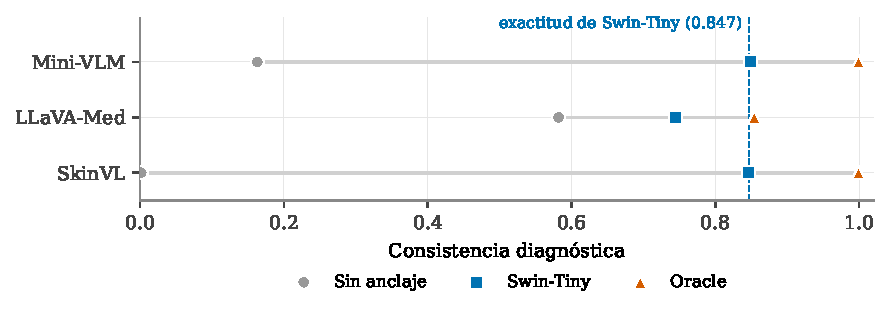
\includegraphics[width=\textwidth]{Figures/Capitulos/05-Resultados-Generacion/cascada-fuentes.pdf}
    \caption{Consistencia diagnóstica de cada generador según la fuente del diagnóstico. La línea discontinua es la
    exactitud de Swin-Tiny.}
    \label{fig:res_gen_cascada}
\end{figure}

\begin{table}[H]
    \centering
    \caption{Consistencia diagnóstica de la cascada según la fuente del diagnóstico, con las diferencias y su IC del
    95\,\% (bootstrap pareado).}
    \label{tab:res_gen_cascada}
    \small
    \setlength{\tabcolsep}{2pt}
    \begin{tabularx}{\textwidth}{@{}>{\raggedright\arraybackslash}X cccccc@{}}
        \toprule
        \textbf{Generador} & \textbf{\encabezado{Sin\\anclaje}} & \textbf{DermLIP} & \textbf{\encabezado{Swin-\\Tiny}}
            & \textbf{Oracle} & \textbf{\encabezado{Swin-Tiny $-$\\sin anclaje}} & \textbf{\encabezado{Oracle $-$\\Swin-Tiny}} \\
        \midrule
        Mini-VLM & 0.163 & 0.717 & 0.849 & 0.999 & $+0.686$ [$+0.658$, $+0.712$] & $+0.150$ [$+0.132$, $+0.168$] \\
        LLaVA-Med & 0.582 & 0.641 & 0.745 & 0.854 & $+0.162$ [$+0.130$, $+0.194$] & $+0.110$ [$+0.094$, $+0.126$] \\
        SkinVL & 0.001 & 0.716 & 0.846 & 0.999 & $+0.845$ [$+0.827$, $+0.863$] & $+0.153$ [$+0.135$, $+0.171$] \\
        \bottomrule
    \end{tabularx}
\end{table}

Que la consistencia coincida con la exactitud del clasificador se explica porque los generadores copian el diagnóstico
que reciben. Mini-VLM nombra el diagnóstico de Swin-Tiny en todos los reportes salvo dos. Cuando ese diagnóstico es
correcto, el reporte nombra la clase verdadera en 1\,272 de 1\,273 imágenes, y cuando es incorrecto, solo en 4 de
230. Por lo tanto, en la cascada la fidelidad diagnóstica del reporte es la exactitud del clasificador, y la distancia
al oracle mide sus errores y no los del generador.

LLaVA-Med es la excepción, porque no siempre transcribe el diagnóstico. Aun con el oracle, uno de cada siete
reportes no nombra la clase recibida. La mayoría describe la lesión y termina sin enunciar ningún diagnóstico, a pesar
de que la instrucción lo pide, y el resto son textos demasiado breves, entre ellos los que quedan vacíos cuando el
límite de tokens corta un bloque de razonamiento. Estas omisiones se concentran en \gls{nv}, \gls{bkl} y \gls{akiec}, y
son fallas del generador y no del clasificador (Sección~\ref{sec:res_gen_errores}).

La misma relación aparece cuando la fuente es DermLIP sin ajuste, el \gls{vlm} de la Sección~\ref{sec:res_vlm}, que
acierta en 0.716 de las imágenes de la prueba. Mini-VLM y SkinVL nombran el diagnóstico de DermLIP en todos los
reportes salvo uno y dos, respectivamente, y su consistencia coincide con esa exactitud. Por lo tanto, el generador
transcribe el diagnóstico de igual modo cuando proviene de un clasificador ajustado y cuando proviene de un modelo
sin ajuste, y la fidelidad del reporte es la de la fuente.

Lo que cambia con la fuente es cuántos errores se transcriben. Con Mini-VLM, la cascada con Swin-Tiny supera a la de
DermLIP en 0.132 [0.107, 0.158] de consistencia, y la diferencia es similar con los otros dos generadores. LLaVA-Med,
además, apenas mejora con DermLIP frente a no anclar, porque sigue omitiendo el diagnóstico recibido en uno de cada
siete reportes. Por lo tanto, de las dos fuentes que no conocen la etiqueta, el clasificador ajustado es la que lleva
más diagnósticos correctos al reporte.

\subsection{Consistencia por clase}
\label{sec:res_gen_clases}

Si el generador copia el diagnóstico, la cascada hereda también la sensibilidad de Swin-Tiny en cada clase. La
Figura~\ref{fig:res_gen_clases} lo confirma: con Mini-VLM y SkinVL, la consistencia de cada clase coincide con la
sensibilidad del clasificador en esa clase, de modo que los puntos quedan sobre la diagonal. LLaVA-Med queda por debajo
en casi todas las clases, y la mayor pérdida está en \gls{akiec}, donde nombra la clase en la mitad de los reportes en
que el clasificador la acierta.

\begin{figure}[H]
    \centering
    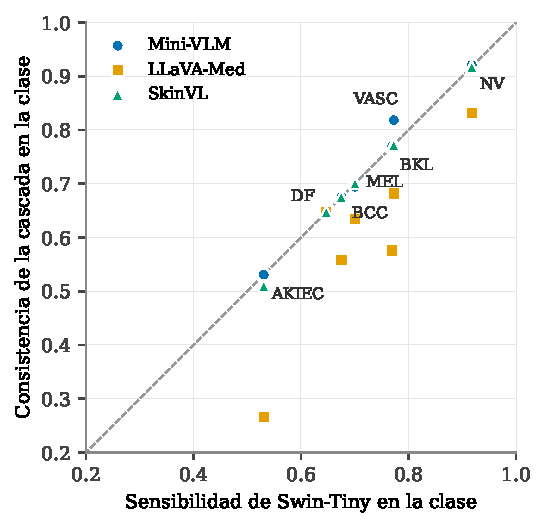
\includegraphics[width=0.62\textwidth]{Figures/Capitulos/05-Resultados-Generacion/cascada-por-clase.pdf}
    \caption{Sensibilidad de Swin-Tiny en cada clase frente a la consistencia de la cascada en esa clase.}
    \label{fig:res_gen_clases}
\end{figure}

La consecuencia clínica es que la cascada reproduce los puntos débiles del clasificador. Con la semilla que ancla el
pipeline, Swin-Tiny reconoce siete de cada diez melanomas, algo más que la media de sus tres semillas
(Sección~\ref{sec:res_melanoma}), y por ello tres
de cada diez reportes de un melanoma no lo nombran. Las clases con menor sensibilidad, como \gls{akiec},
reciben del mismo modo los reportes menos fieles, de modo que mejorar el reporte de una clase exige mejorar el
diagnóstico que lo ancla.

\subsection{Aporte de la imagen al reporte}
\label{sec:res_gen_ablaciones}

Si la fidelidad del reporte viene del clasificador, queda por saber qué hace el generador con la imagen. Para
responderlo, la cascada con el oracle se repitió en las dos variantes de la
Sección~\ref{sec:met_referencias}: con la imagen reemplazada por una gris neutra y con un diagnóstico equivocado, como
\gls{mel} por \gls{nv}. La Tabla~\ref{tab:res_gen_ablaciones} reúne los resultados, sobre 400 imágenes con Mini-VLM y
LLaVA-Med y sobre la prueba completa con SkinVL.

\begin{table}[H]
    \centering
    \caption{Cascada con el oracle con la imagen, sin ella y con un diagnóstico equivocado. La consistencia se
    mide respecto de la clase verdadera.}
    \label{tab:res_gen_ablaciones}
    \small
    \setlength{\tabcolsep}{3pt}
    \begin{tabularx}{\textwidth}{@{}>{\raggedright\arraybackslash}X cccccc@{}}
        \toprule
        & & \multicolumn{3}{c}{\textbf{Consistencia diagnóstica}} & \textbf{\encabezado{Reportes\\distintos}}
            & \textbf{\encabezado{Cobertura\\de entidades}} \\
        \cmidrule(lr){3-5}
        \textbf{Generador} & \textbf{Imágenes} & \textbf{\encabezado{Con\\imagen}} & \textbf{\encabezado{Sin\\imagen}}
            & \textbf{\encabezado{Diagnóstico\\equivocado}} & \textbf{\encabezado{Con / sin\\imagen}}
            & \textbf{\encabezado{Con / sin\\imagen}} \\
        \midrule
        Mini-VLM & 400 & 1.000 & 1.000 & 0.000 & 395 / 7 & 0.787 / 0.378 \\
        LLaVA-Med & 400 & 0.863 & 0.893 & 0.020 & 399 / 7 & 0.760 / 0.811 \\
        SkinVL & 1\,503 & 0.999 & 0.967 & 0.000 & 67 / 7 & 0.377 / 0.423 \\
        \bottomrule
    \end{tabularx}
\end{table}

La imagen no interviene en qué diagnóstico afirma el reporte. Sin ella, la consistencia no cambia con Mini-VLM, con
LLaVA-Med sube tres centésimas sin que la diferencia se distinga de cero, y con SkinVL baja apenas tres centésimas. Con un diagnóstico equivocado, en cambio, la consistencia cae a
cero en los tres generadores, porque el reporte afirma el diagnóstico recibido y no lo corrige a partir de la imagen:
Mini-VLM nombra la clase equivocada en todos los reportes y LLaVA-Med, en tres de cada cuatro. En consecuencia, un
error del clasificador llega al reporte sin ninguna corrección.

La imagen sí interviene en qué se describe. Sin ella, los tres generadores escriben un único texto por clase, siete
por generador, mientras que con ella casi cada reporte de Mini-VLM y de LLaVA-Med es distinto. Además, la cobertura de entidades
clínicas de Mini-VLM cae a la mitad sin la imagen, de modo que su descripción se apoya en ella. En LLaVA-Med, en cambio,
la cobertura no baja, porque sin la imagen el generador escribe una descripción genérica de la clase, con tantos
términos clínicos como la de una lesión concreta. Por lo tanto, el clasificador aporta el diagnóstico, y la imagen
aporta la variación de la descripción entre lesiones, aunque estas métricas no permiten saber si lo descrito está en la imagen
(Sección~\ref{sec:met_eval_generacion}).

\subsection{Fallas de los reportes}
\label{sec:res_gen_errores}

La consistencia indica si el reporte nombra la clase verdadera, pero no de qué manera falla cuando no lo hace. Para
saberlo, cada reporte se asignó a su falla principal con las reglas de la Sección~\ref{sec:met_eval_generacion}, que
cuentan aparte la expresión de reserva junto a la clase verdadera, como «consistent with nevus», porque el reporte se
compromete con el diagnóstico. La Figura~\ref{fig:res_gen_errores} muestra la distribución de las fallas de cada
generador sin anclaje, con Swin-Tiny y con el oracle.

\begin{figure}[H]
    \centering
    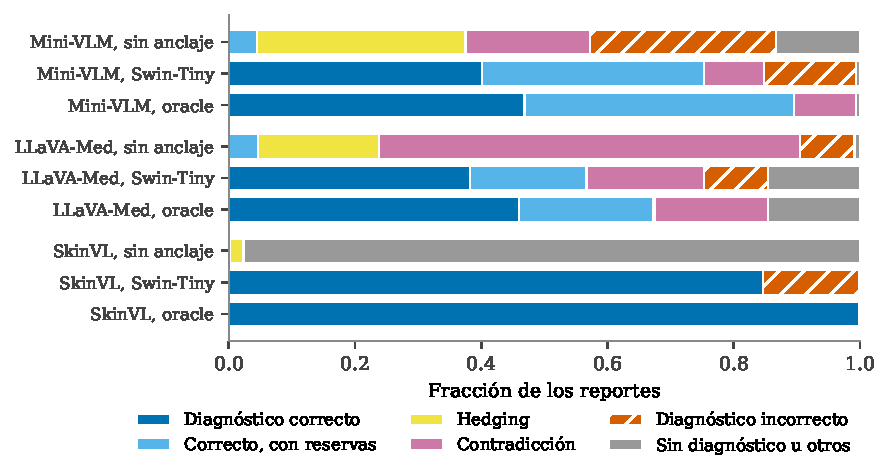
\includegraphics[width=\textwidth]{Figures/Capitulos/05-Resultados-Generacion/fallas-reportes.pdf}
    \caption{Falla principal de los reportes de cada generador según la fuente del diagnóstico.}
    \label{fig:res_gen_errores}
\end{figure}

Sin anclaje, cada generador tiene un patrón de fallas distinto. Dos de cada tres reportes de LLaVA-Med son contradicciones,
porque enumeran varias clases, y Mini-VLM reparte sus fallas entre el hedging y el diagnóstico incorrecto, que
juntos reúnen casi dos tercios de sus reportes. SkinVL, por su parte, no nombra ninguna clase en casi ningún reporte.
Estas distribuciones explican las consistencias de la Tabla~\ref{tab:res_gen_sin_anclaje}: la de LLaVA-Med proviene
de enumerar y no de afirmar el diagnóstico.

Con el anclaje, el hedging desaparece en los tres generadores, y el diagnóstico incorrecto queda reducido a los
errores del clasificador. Con el oracle, el diagnóstico incorrecto desaparece, y lo que queda son fallas del
generador. En Mini-VLM, uno de cada diez reportes nombra además otra clase, mientras que en LLaVA-Med casi uno de cada
cinco es una contradicción y uno de cada diez no nombra ninguna clase. SkinVL no tiene más fallas que las del
clasificador, porque escribe una oración breve con el diagnóstico recibido. La repetición, frecuente con la
decodificación voraz (Sección~\ref{sec:marco_rep_fallas}), afecta al 4\,\% de los reportes de Mini-VLM sin anclaje y a
menos del 1\,\% con anclaje.

\subsection{Recuperación de casos parecidos}
\label{sec:res_gen_rag}

La cascada depende de un clasificador entrenado, y la recuperación de la Sección~\ref{sec:met_recuperacion} es la
alternativa que entrega al generador los diagnósticos de los tres casos de entrenamiento más parecidos. La
Tabla~\ref{tab:res_gen_rag} la compara con la cascada en Mini-VLM, junto con dos líneas base sin generador que
escriben solo el diagnóstico: el voto del \gls{knn} y el de Swin-Tiny. Además de la consistencia, la tabla informa la
proporción de reportes que nombran la clase verdadera y ninguna otra.

\begin{table}[H]
    \centering
    \caption{Recuperación frente a la cascada en Mini-VLM.}
    \label{tab:res_gen_rag}
    \small
    \begin{tabularx}{\textwidth}{@{}>{\raggedright\arraybackslash}X >{\centering\arraybackslash}p{3.0cm}
        >{\centering\arraybackslash}p{3.0cm}@{}}
        \toprule
        \textbf{Condición} & \textbf{Consistencia diagnóstica} & \textbf{Solo la clase verdadera} \\
        \midrule
        Sin anclaje & 0.163 & 0.045 \\
        Recuperación sola & 0.669 & 0.500 \\
        Voto del \gls{knn}, sin generador & 0.781 & 0.781 \\
        Cascada con Swin-Tiny & 0.849 & 0.757 \\
        Swin-Tiny, sin generador & 0.847 & 0.847 \\
        Cascada con Swin-Tiny y recuperación & 0.862 & 0.792 \\
        \bottomrule
    \end{tabularx}
\end{table}

La recuperación sola mejora mucho la consistencia frente a no anclar, pero no reemplaza al clasificador. Queda casi
dos décimas por debajo de la cascada con Swin-Tiny, y también por debajo de escribir directamente el voto del
\gls{knn}. Es decir, el generador aprovecha peor la información de los vecinos que una regla de votación: cuando los
tres no coinciden, nombra varias clases o una distinta, y por eso solo la mitad de sus reportes nombra únicamente la
clase verdadera.

Sumar la recuperación a la cascada, por su parte, aporta poco. La consistencia sube 0.013 [0.007, 0.019], pero la
ganancia viene de que el reporte agrega la clase de los vecinos cuando difiere de la del clasificador, de modo que
nombra más candidatos: escribir solo el diagnóstico de Swin-Tiny da reportes más exclusivos. Tampoco un vecino
equivocado degrada el reporte. En las 171 imágenes en que Swin-Tiny acierta y el voto del \gls{knn} no, la cascada con
recuperación nombra la clase verdadera en todos los reportes, igual que sin ella, y en las 72 en que ocurre lo
contrario, recupera la clase verdadera en una de cada seis. El generador, por lo tanto, sigue al diagnóstico del
clasificador también cuando recibe otra evidencia.

En síntesis, la cascada lleva al reporte la exactitud del clasificador junto con sus errores, y ni la imagen ni los
casos recuperados corrigen esos errores. La sección siguiente evalúa si la concordancia entre el clasificador y el
\gls{knn} permite reconocer los casos en que el diagnóstico es menos confiable.

% Extensión estimada: unas 6 páginas, dos subsecciones, una tabla y dos figuras (ficha 5.3).
% Fuentes: cap5_derivados.json ("ruteo"), ensemble_bootstrap{,_llava_med}_les_report_only_strict.json
% ("tab_incertidumbre_e2e"), uncertainty_analysis{,_llava_med}_les.json (taxonomía por nivel, abstenidas);
% Codigo/docs/ejecuciones.md, 18/10/2026 (bloques <think> sin cerrar de LLaVA-Med en el diferencial: 144 de 248).
% Cohorte completa: aciertos del pipeline (0.901 × 1 452 = 1 308; LLaVA-Med 0.744 × 1 452 = 1 080) sobre 1 503.
% Figuras: scripts/figuras_cap5.py (ruteo-niveles); ejemplos-reportes.tex.
% Revisión del tutor del 26/10/2026: el ruteo se nombra con su referencia al Capítulo 3 sin volver a describirlo;
% esquema contexto → objeto → valores → conjetura.
\section{Pipeline completo}
\label{sec:res_gen_incertidumbre}

En la cascada, el reporte suele afirmar el diagnóstico del clasificador, aunque sea incorrecto, y ni la imagen ni los vecinos lo corrigen en la mayoría de los casos. El último paso del recorrido agrega el ruteo por concordancia de la Sección~\ref{sec:met_ruteo}, que
completa el \emph{pipeline} de la Figura~\ref{fig:met_pipeline} del Capítulo~\ref{cp:metodos}: según coincidan o no
Swin-Tiny y el \gls{knn}, cada imagen recibe un reporte afirmativo, un reporte diferencial con dos candidatos o se
deriva a un especialista, según los tres niveles de la Tabla~\ref{tab:met_niveles} del Capítulo~\ref{cp:metodos}.

Esta sección presenta los resultados del ruteo en dos partes. La primera evalúa si la concordancia separa los casos en
que el clasificador acierta de aquellos en que se equivoca. La segunda mide cuánto cambian los reportes de Mini-VLM y
LLaVA-Med frente a la cascada simple de la sección anterior y a la línea base sin generador de la
Sección~\ref{sec:met_referencias}.

\subsection{Concordancia entre el clasificador y el kNN}
\label{sec:res_gen_concordancia}

El ruteo asigna ocho de cada diez imágenes del conjunto de prueba al nivel afirmativo, una de cada seis al diferencial y una
de cada treinta a la derivación. Para ver si esos niveles reúnen casos de dificultad distinta, la Figura~\ref{fig:res_gen_ruteo} presenta dos paneles. El
panel (a) indica, en cada nivel, la fracción de casos en que Swin-Tiny acierta y en que el par de candidatos contiene la
clase verdadera. El panel (b) reparte las imágenes de cada clase entre los tres niveles.

\begin{figure}[H]
    \centering
    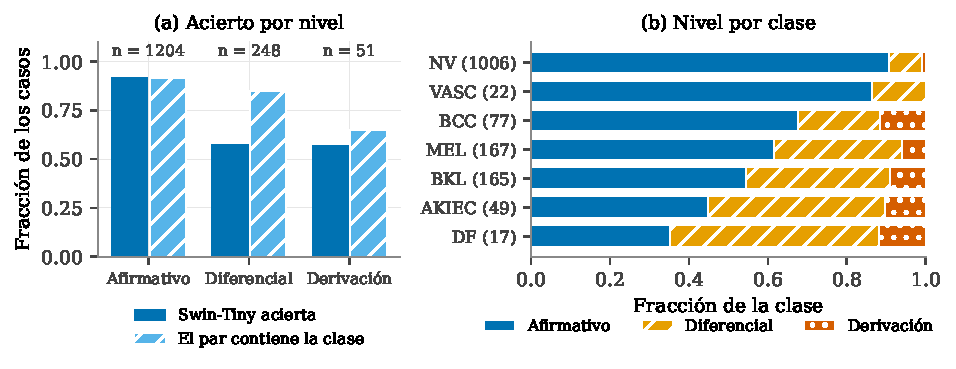
\includegraphics[width=\textwidth]{Figures/Capitulos/05-Resultados-Generacion/ruteo-niveles.pdf}
    \caption{(a) Acierto de Swin-Tiny y del par de candidatos en cada nivel del ruteo; (b) nivel asignado a las
    imágenes de cada clase, con el número de imágenes entre paréntesis.}
    \label{fig:res_gen_ruteo}
\end{figure}

Swin-Tiny acierta el 91.5\,\% de los casos afirmativos y poco más de la mitad de los otros dos niveles. En este conjunto de prueba, la concordancia discrimina subconjuntos con diferentes tasas de error, como suponía el diseño del ruteo (Sección~\ref{sec:met_ruteo}), y su transferencia a otros conjuntos debe evaluarse aparte. Tampoco proporciona una estimación calibrada de confianza para cada caso.

En el nivel diferencial, presentar los dos candidatos cubre muchos más casos que el diagnóstico del clasificador
solo. El par formado por la clase de Swin-Tiny y el voto del \gls{knn} contiene la clase verdadera en el 84.7\,\% de
esos casos, frente al 57.3\,\% del clasificador. El voto del \gls{knn} acierta en ellos con menos frecuencia que
Swin-Tiny, pero, como en este nivel los dos predictores difieren, cada acierto del \gls{knn} corresponde a un error
del clasificador, y eso es lo que justifica usarlo como segunda opinión.

La concordancia, sin embargo, no detecta los errores que comparten ambos predictores. De los 230 casos en que
Swin-Tiny se equivoca, 102 caen en el nivel afirmativo, porque el \gls{knn} vota la misma clase errónea. Es decir,
cuatro de cada nueve errores del clasificador se afirman con la misma plantilla que un acierto, la limitación que
anticipaba la Sección~\ref{sec:met_ruteo}. El caso más relevante es el melanoma: 38 de los 167 melanomas del conjunto de prueba
se afirman como otra clase, 31 de ellos como \gls{nv}, de modo que casi uno de cada cuatro melanomas recibe un
reporte definitivo con un diagnóstico benigno.

Por clase, el panel (b) muestra que el ruteo afirma casi todos los \gls{nv} y las lesiones vasculares, y deriva o
presenta como diferencial más de la mitad de las imágenes de \gls{df} y de \gls{akiec}. El melanoma queda en una
posición intermedia. Un tercio de los melanomas va al nivel diferencial, y en ese caso el par de candidatos contiene el
melanoma en 52 de 54 imágenes, la mayoría como par melanoma--nevo, la confusión más costosa según la
Sección~\ref{sec:met_seleccion}.

La derivación, por último, deja fuera del \emph{pipeline} 51 casos en los que el clasificador acierta tan poco como en
el nivel diferencial. Esta decisión tiene un costo: en esos casos, con la cascada simple, Mini-VLM habría escrito 20
reportes con un diagnóstico incorrecto y dos con una contradicción, mientras que el clasificador acierta 29 de los 51
diagnósticos, que la derivación también descarta. Por eso la derivación evita errores y deja sin reporte 29 diagnósticos correctos, y su utilidad depende de cuánto cueste en la práctica un error frente a una consulta con el
especialista.

\subsection{Reportes del pipeline completo}
\label{sec:res_gen_pipeline}

Con el ruteo, los casos afirmativos reciben el reporte de la cascada y los diferenciales, uno que discute los dos
candidatos. La Tabla~\ref{tab:res_gen_pipeline} compara la consistencia de esos reportes, para Mini-VLM y LLaVA-Med
(columnas), en tres bloques de filas. El primero reúne los 1\,452 casos no derivados, con la cascada simple, el
\emph{pipeline}, la línea base sin generador, que escribe el diagnóstico afirmado o el par de candidatos, y las
diferencias pareadas con su intervalo de confianza. El segundo se limita al nivel diferencial, y el tercero vuelve al conjunto de prueba completo, con cada derivación contada como un caso sin diagnóstico.

Esta consistencia no equivale a una exactitud, por dos razones. Primero, en el nivel diferencial un reporte que nombra
dos candidatos cuenta como consistente si uno de ellos es el verdadero, de modo que el criterio se parece a acertar
entre las dos primeras opciones. Segundo, la consistencia de los casos no derivados excluye las derivaciones, que son
de los más difíciles, y por eso el tercer bloque informa también la consistencia sobre las 1\,503 imágenes.

\begin{table}[H]
    \centering
    \caption{Consistencia diagnóstica del pipeline completo frente a la cascada simple y a la línea base sin
    generador. Entre corchetes, el intervalo de confianza (IC) del 95\,\% de cada diferencia, estimado con \emph{bootstrap} pareado (Sección~\ref{sec:met_estadistica}); una diferencia cuyo IC no incluye el cero es estadísticamente significativa. En negrita, el mayor valor de cada bloque y las diferencias cuyo IC no incluye el cero.}
    \label{tab:res_gen_pipeline}
    \small
    \setlength{\tabcolsep}{4pt}
    \begin{tabularx}{\textwidth}{@{}>{\raggedright\arraybackslash}X cc@{}}
        \toprule
        & \textbf{Mini-VLM} & \textbf{LLaVA-Med} \\
        \midrule
        \multicolumn{3}{@{}l}{\textit{Casos no derivados (1\,452)}} \\
        Cascada simple & 0.858 & 0.755 \\
        Pipeline completo & 0.901 & 0.744 \\
        Línea base sin generador & \textbf{0.904} & \textbf{0.904} \\
        Pipeline $-$ cascada simple & $\mathbf{+0.043}$ [$+0.031$, $+0.055$] & $-0.011$ [$-0.025$, $+0.003$] \\
        Pipeline $-$ línea base sin generador & $-0.003$ [$-0.008$, $+0.002$] & $\mathbf{-0.160}$ [$-0.180$, $-0.140$] \\
        \filasep
        \multicolumn{3}{@{}l}{\textit{Nivel diferencial (248)}} \\
        Cascada simple & 0.581 & 0.472 \\
        Reporte diferencial & 0.831 & 0.407 \\
        Par de candidatos, sin generador & \textbf{0.847} & \textbf{0.847} \\
        \filasep
        \multicolumn{3}{@{}l}{\textit{Conjunto de prueba completo, con las derivaciones sin diagnóstico (1\,503)}} \\
        Cascada simple & 0.849 & 0.745 \\
        Pipeline completo & 0.870 & 0.719 \\
        Línea base sin generador & \textbf{0.873} & \textbf{0.873} \\
        \bottomrule
    \end{tabularx}
\end{table}

La línea base sin generador obtiene la consistencia más alta en los tres bloques, y LLaVA-Med en el \emph{pipeline},
la más baja. Con Mini-VLM, el \emph{pipeline} obtiene una mayor consistencia diagnóstica que la cascada simple según la métrica utilizada. Esta mejora se concentra en el nivel diferencial, donde el reporte nombra la clase verdadera en cuatro de cada cinco casos, frente a seis de cada diez de la cascada. En ese nivel se consideran consistentes los reportes que incluyen la clase verdadera entre dos candidatos, por lo que la mejora no equivale directamente a un aumento de la exactitud diagnóstica. Sin embargo, el \emph{pipeline} no supera a la línea base sin generador. La ganancia puede atribuirse, por lo tanto, a presentar dos candidatos cuando los predictores discrepan, una decisión del ruteo, y el generador la
conserva sin agregarle fidelidad. Sobre el conjunto de prueba completo, con las derivaciones contadas como casos sin diagnóstico,
la mejora es menor, de 0.849 a 0.870. Esta lectura coincide con la de la cascada: el diagnóstico sale de los
predictores, y el generador lo redacta.

Con LLaVA-Med, en cambio, el \emph{pipeline} no mejora la cascada simple, y sobre el conjunto de prueba completo queda por debajo de
ella. Sus reportes diferenciales nombran la clase verdadera en cuatro de cada diez casos, la mitad que el par de
candidatos que reciben. En 144 de los 248, el generador abre un bloque de razonamiento que el límite de tokens deja sin
cerrar, y los candidatos quedan dentro de él. Como la evaluación mide solo el reporte
(Sección~\ref{sec:met_eval_generacion}), esos candidatos no cuentan. Una explicación posible es que la plantilla
diferencial, que pide discutir dos candidatos, induce a LLaVA-Med a razonar, mientras que la plantilla
\emph{noreasoning} del nivel afirmativo lo evita en general.

Según la clasificación de fallas de la Sección~\ref{sec:res_gen_errores}, disminuye también la proporción de reportes con un diagnóstico incorrecto, es decir, que nombran otra clase y no la verdadera. Entre los 1\,452 casos no derivados, bajan del 13.6\,\% al 9.0\,\% con Mini-VLM y del 9.4\,\% al 7.1\,\% con LLaVA-Med, si en el nivel diferencial se cuenta como
correcto el reporte que incluye la clase verdadera entre los dos candidatos. Esta reducción refleja en parte la presentación de diagnósticos alternativos y no debe interpretarse directamente como una disminución equivalente del riesgo clínico. El precio es un formato menos estable, ya que
los reportes diferenciales de Mini-VLM nombran en promedio más de dos clases y los reportes con repeticiones internas pasan de 7 a 48 de los 1\,452 casos no derivados.

Las métricas anteriores no muestran cómo se lee un reporte. Para completarlas con un análisis cualitativo, la
Figura~\ref{fig:res_gen_ejemplos} reúne tres reportes de
Mini-VLM en el \emph{pipeline}, uno por situación, citados en inglés. En el primero, el clasificador y los vecinos coinciden en
melanoma, y el reporte afirma el diagnóstico de melanoma y menciona características habitualmente asociadas con esa categoría, como bordes irregulares y asimetría.

El segundo es un caso diferencial: el clasificador predice melanoma, dos de los tres vecinos son nevos, y el reporte
discute los dos candidatos y recomienda una biopsia. El texto incluye, sin embargo, una oración que repite la
instrucción recibida («The final clinical report should include…»), un defecto de redacción que las métricas
automáticas no detectan. El tercero es un error compartido: el clasificador y los tres vecinos coinciden en nevo para
un melanoma, y el reporte afirma el nevo y describe una pigmentación homogénea «with no visible melanocytic infiltration or atypical features». Es decir, la
descripción acompaña al diagnóstico recibido, y un error del clasificador llega al reporte con rasgos que lo hacen
verosímil.

En conjunto, el ruteo identifica una parte de los casos dudosos y, en ellos, presentar dos candidatos cubre más que
afirmar uno, aunque los errores compartidos por los dos predictores se siguen afirmando. La sección siguiente compara
los tres generadores con estos resultados y con su costo de ejecución.

% Tres reportes reales de Mini-VLM (configuración principal), elegidos con scripts de lectura sobre
% outputs/generated_reports/mini_vlm/{full_swin_les,full_differential_les}: el nivel afirmativo con el diagnóstico
% correcto, el diferencial con el par {Swin-Tiny, kNN} y el afirmativo con un error compartido. Imágenes de HAM10000
% (CC BY-NC 4.0), recortadas al centro, reducidas a 300 px y guardadas como PDF (el .gitignore excluye los JPG de
% Docs/). Los «[...]» marcan texto omitido.
\begin{figure}[H]
    \centering
    \footnotesize
    \newcommand{\ejemplo}[3]{%
        \begin{minipage}[c]{0.2\textwidth}
            \centering
            \includegraphics[width=\textwidth]{Figures/Capitulos/05-Resultados-Generacion/ejemplo-#1.pdf}
        \end{minipage}\hfill
        \begin{minipage}[c]{0.77\textwidth}
            \raggedright #2\par\smallskip
            \itshape #3
        \end{minipage}}
    \ejemplo{ISIC_0029473}{(a) Afirmativo. Clase verdadera: \gls{mel}. Swin-Tiny: \gls{mel}; los tres vecinos:
        \gls{mel}.}{«Final Clinical Report: Diagnosis - Melanoma. Morphological features include a
        pigmented lesion with irregular borders and an asymmetrical shape. Dermatoscopic examination reveals atypical
        melanocytic proliferation with irregular pigmentation patterns.»}
    \par\medskip\hrule\medskip
    \ejemplo{ISIC_0031194}{(b) Diferencial. Clase verdadera: \gls{nv}. Swin-Tiny: \gls{mel}; vecinos: \gls{mel},
        \gls{nv}, \gls{nv}.}{«The lesion in question presents with a well-defined, irregular border and a
        brownish-black coloration, which are characteristic features of melanoma. However, the presence of a central
        depression and the overall morphology could also suggest a nevus [\ldots] The final clinical report should
        include a detailed description of the lesion's morphological and dermatoscopic features, presenting these as
        a differential diagnosis between melanoma and nevus. Further diagnostic steps, such as a biopsy, may be
        necessary to confirm the diagnosis and rule out malignancy.»}
    \par\medskip\hrule\medskip
    \ejemplo{ISIC_0033452}{(c) Afirmativo con un error compartido. Clase verdadera: \gls{mel}. Swin-Tiny: \gls{nv};
        vecinos: \gls{nv}, \gls{nv}, \gls{nv}.}{«Final Clinical Report: The diagnosis is nevus. The lesion is
        characterized by a well-defined, brown, macular area with a smooth border and a slightly elevated surface.
        Dermatoscopic examination reveals a homogeneous pigmentation with no visible melanocytic infiltration or
        atypical features.»}
    \caption[Reportes de Mini-VLM en el \emph{pipeline}]{Reportes de Mini-VLM en el \emph{pipeline}, uno por
    situación. Imágenes de \emph{HAM10000}~\cite{tschandl2018ham10000}, licencia CC BY-NC 4.0.}
    \label{fig:res_gen_ejemplos}
\end{figure}


% Extensión estimada: unas 4 páginas, dos subsecciones, dos tablas y una figura (ficha 5.4).
% Fuentes: cap5_derivados.json ("entre_generadores", "fallas": cobertura, palabras y reportes distintos con Swin-Tiny);
% ensemble_bootstrap*_les_report_only_strict.json; Codigo/docs/resul/mini_vlm_lora_llm_resul_v3_20261024.md (control,
% parcial: Swin-Tiny 963 de 1 503, sin anclaje 372); cost/cost_comparison_v3.json (segundos por reporte, de las
% corridas del re-anclaje en la A30; parámetros); logs 1153597 y 1153598 (segunda etapa: 9 h 21 min y 6 h 55 min).
% Memoria y parámetros medidos en la A30: cost/vlm_memory_<gen>.json (scripts/measure_vlm_memory.py, Mendieta
% 1183335–37; torch.cuda.max_memory_allocated en GiB, 20 reportes de la cascada). Nivel 1 pareado de la variante de
% control: level1_test/skincot_test_mini_v2/level1_pareado_mini_v2_v3_llava_v2.json (n = 349).
% Figura: scripts/figuras_cap5.py (resumen-generadores).
% El label del costo es sec:res_costo (lo cita el Capítulo 6).
\section{Comparación entre los generadores}
\label{sec:res_gen_comparacion}

Las secciones anteriores siguieron sobre todo a Mini-VLM, la configuración principal, y mencionaron a los otros
generadores donde se comportan distinto. Puestos en una misma escala, la Figura~\ref{fig:res_gen_resumen} reúne lo que
separa a los tres con el diagnóstico de Swin-Tiny: la consistencia diagnóstica, la cobertura de entidades clínicas y el
tiempo por reporte.

\begin{figure}[H]
    \centering
    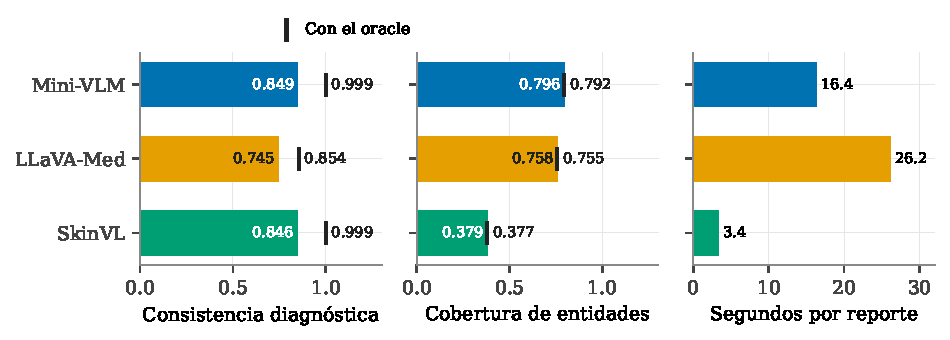
\includegraphics[width=\textwidth]{Figures/Capitulos/05-Resultados-Generacion/resumen-generadores.pdf}
    \caption{Consistencia diagnóstica, cobertura de entidades clínicas y tiempo por reporte de los tres generadores
    en la cascada con Swin-Tiny. La marca vertical es la consistencia con el \emph{oracle}.}
    \label{fig:res_gen_resumen}
\end{figure}

En consistencia, Mini-VLM y SkinVL no se distinguen, ni con Swin-Tiny ni con el \emph{oracle}, porque los dos copian el
diagnóstico. Mini-VLM supera a LLaVA-Med por una décima con Swin-Tiny, 0.104 [0.087, 0.122], y la diferencia crece con
el \emph{oracle}, porque en ese caso todas las fallas son del generador. Es decir, el generador biomédico más grande es
el que menos transcribe el diagnóstico recibido.

La cobertura de entidades separa a SkinVL de los otros dos. Sus reportes tienen una mediana de 17 palabras, frente a 62
de Mini-VLM y 86 de LLaVA-Med, y cubren la mitad de las entidades clínicas. Además, con Swin-Tiny escribe solo 59
reportes distintos para las 1\,503 imágenes, de modo que su texto depende del diagnóstico y casi nada de la imagen. Por
lo tanto, la especialización en dermatología no mejora la fidelidad del reporte, que ya fija el clasificador, y reduce
la descripción, que es lo que el generador agrega en la cascada. Mini-VLM, en cambio, iguala la fidelidad de SkinVL y
describe tanto como LLaVA-Med, y por eso es el generador de referencia del trabajo.

\subsection{Ajuste del modelo de lenguaje de Mini-VLM}
\label{sec:res_gen_control_mini}

En la configuración principal, Mini-VLM aprende a redactar sin que se ajuste su modelo de lenguaje
(Sección~\ref{sec:met_generacion}). La variante de control, que también ajusta ese modelo, permite saber si esa
decisión cambia los reportes. La Tabla~\ref{tab:res_gen_control} compara ambas versiones sobre las mismas imágenes en
cada fuente de diagnóstico; en la cascada con Swin-Tiny y sin anclaje, la variante de control tiene reportes solo para
una parte de la prueba.

\begin{table}[H]
    \centering
    \caption{Consistencia diagnóstica de la variante de control de Mini-VLM frente a la configuración principal, con
    IC del 95\,\% (\emph{bootstrap} pareado).}
    \label{tab:res_gen_control}
    \small
    \begin{tabularx}{\textwidth}{@{}>{\raggedright\arraybackslash}X cccc@{}}
        \toprule
        \textbf{Fuente del diagnóstico} & \textbf{Imágenes} & \textbf{Control} & \textbf{Principal}
            & \textbf{Diferencia} \\
        \midrule
        \emph{Oracle} & 1\,503 & 0.967 & 0.999 & $-0.033$ [$-0.042$, $-0.023$] \\
        Swin-Tiny & 963 & 0.843 & 0.850 & $-0.007$ [$-0.021$, $+0.006$] \\
        Sin anclaje & 372 & 0.196 & 0.185 & $+0.011$ [$-0.043$, $+0.065$] \\
        Nivel diferencial & 248 & 0.863 & 0.831 & $+0.032$ [$-0.008$, $+0.077$] \\
        \bottomrule
    \end{tabularx}
\end{table}

Ajustar el modelo de lenguaje no cambia la cascada con Swin-Tiny ni el nivel diferencial, y en la generación sin
anclaje tampoco mejora la consistencia. Lo que sí cambia es el formato: la variante de control aprende la estructura de
\emph{SkinCoT} y abre bloques de razonamiento en uno de cada cuatro reportes de \emph{HAM10000}. Con el \emph{oracle},
esa estructura le cuesta tres centésimas de consistencia, porque en parte de los reportes el límite de 384 tokens llega
antes de que el diagnóstico salga del razonamiento.

En \emph{SkinCoT}, el mismo efecto es mayor. La variante de control abre un bloque de razonamiento en casi dos de cada
tres reportes, y uno de cada seis queda vacío al quitarlo. Sobre los 349 pares en que ambos generadores escriben un
reporte, además, el parecido con la referencia cambia poco y en sentidos opuestos según la métrica: la variante de
control supera a la principal en BLEU-4 y en BERTScore, 0.781 frente a 0.770, y queda por debajo en ROUGE-L y METEOR,
mientras que las dos quedan por debajo de LLaVA-Med en las cinco. Por lo tanto, ajustar el modelo de lenguaje acerca el
formato al de \emph{SkinCoT} sin mejorar la fidelidad ni, de manera consistente, el parecido con la referencia, a
costa de reportes vacíos, y la configuración principal se mantiene.

\subsection{Costo computacional del pipeline}
\label{sec:res_costo}

El costo de los clasificadores, que se mide en milisegundos por imagen (Sección~\ref{sec:res_costo_clasificadores}),
es una parte mínima del costo del \emph{pipeline}. La Tabla~\ref{tab:res_costo_generadores} reúne el de los
generadores: el tiempo del ajuste, el tiempo por reporte en la A30 de la Sección~\ref{sec:met_entorno}, con la
cascada y el límite de 384 tokens, y el tiempo que llevaría generar los reportes de toda la prueba. La memoria es la
máxima ocupada por los tensores en la GPU, medida al cargar el modelo y durante la generación de 20 reportes de la
cascada.

\begin{table}[H]
    \centering
    \caption{Costo de los generadores, medido en la A30.}
    \label{tab:res_costo_generadores}
    \small
    \setlength{\tabcolsep}{3pt}
    \begin{tabularx}{\textwidth}{@{}>{\raggedright\arraybackslash}X
        >{\centering\arraybackslash}p{1.9cm}>{\centering\arraybackslash}p{1.6cm}>{\centering\arraybackslash}p{1.9cm}
        >{\centering\arraybackslash}p{1.9cm}>{\centering\arraybackslash}p{1.7cm}>{\centering\arraybackslash}p{1.7cm}@{}}
        \toprule
        & & \multicolumn{2}{c}{\textbf{Memoria (GB)}} & & & \\
        \cmidrule(lr){3-4}
        \textbf{Generador} & \textbf{Parámetros (millones)} & \textbf{Carga} & \textbf{Generación}
            & \textbf{Ajuste, segunda etapa (h)} & \textbf{Segundos por reporte} & \textbf{Horas para la prueba} \\
        \midrule
        Mini-VLM & 4\,153 & 7.7 & 8.6 & 9.3 & 16.4 & 6.8 \\
        LLaVA-Med & 7\,600 & 14.2 & 14.5 & 6.9 & 26.2 & 10.9 \\
        SkinVL & 7\,567 & 14.1 & 14.4 & --- & 3.4 & 1.4 \\
        \bottomrule
    \end{tabularx}
\end{table}

Un reporte de Mini-VLM tarda unas mil quinientas veces más que una clasificación de Swin-Tiny, de modo que el costo del
\emph{pipeline} lo fija el generador. El \gls{knn} tampoco cambia esa cuenta, porque requiere una pasada del
codificador de DermLIP, un ViT-B/16 como el clasificador del mismo nombre de la
Tabla~\ref{tab:res_costo_clasificadores}, y una búsqueda entre 6\,447 \emph{embeddings}. Entre los generadores, el
tiempo por reporte depende más de lo que escriben que de su tamaño: SkinVL, del mismo tamaño que LLaVA-Med, es el más
rápido porque escribe una oración, y Mini-VLM tarda menos que LLaVA-Med con reportes más breves.

La memoria, en cambio, sí depende del tamaño. Mini-VLM ocupa como máximo 8.6~GB durante la generación, por debajo de
los 12~GB de una GPU de consumo como la RTX 4070, mientras que LLaVA-Med y SkinVL superan esa cifra ya al cargar los
pesos. La generación agrega poco a la carga, porque cada reporte se escribe de a uno y con un límite de 384 tokens. El ajuste de Mini-VLM tomó
algo más de nueve horas en una sola GPU, y el de LLaVA-Med, algo menos de siete. Por lo tanto, el \emph{pipeline} con
Mini-VLM cumple la restricción de cómputo de la Sección~\ref{sec:met_tareas}: se ajusta y se ejecuta en una sola GPU,
con un reporte en menos de 20 segundos, y la comparación con el cómputo que usan los trabajos revisados se retoma en el
Capítulo~\ref{cp:discusion}.

% Extensión estimada: unas 2 páginas, cuatro párrafos y una tabla (ficha 5.5).
% Fuentes: Tablas tab:marco_generadores y tab:marco_sota_reportes y Sección 2.7.3 (sec:estado_arte_reportes) del
% Capítulo 2; Zeng et al., MM-Skin, Tabla 3 (VQA, columna de dermatoscopía, escala 0--100; verificada en el PDF el
% 24/10/2026): LLaVA-Med-7B BLEU-4 8.88, BERTScore 66.60; SkinVL-MM 21.61 y 71.34. Cifras propias de las
% secciones 5.1 a 5.4.
\section{Comparación con el estado del arte}
\label{sec:res_gen_estado_arte}

Como en la clasificación (Sección~\ref{sec:res_estado_arte}), los trabajos de generación de reportes del
Capítulo~\ref{cp:marco} usan otros datos, otras instrucciones y, sobre todo, otras formas de evaluar el texto, de modo
que la comparación ubica el orden de magnitud de los resultados y no ordena los sistemas. La
Tabla~\ref{tab:res_gen_estado_arte} reúne las cifras que tienen un equivalente en este trabajo, en tres bloques: el
parecido con un texto de referencia, la corrección del diagnóstico en el texto y el efecto del contexto recuperado.

\begin{table}[htbp]
    \centering
    \caption{Resultados de la literatura (Capítulo~\ref{cp:marco}) frente a los de este trabajo, en escala de 0 a 1.
    «---»: sin cifra equivalente.}
    \label{tab:res_gen_estado_arte}
    \footnotesize
    \setlength{\tabcolsep}{3pt}
    \begin{tabularx}{\textwidth}{@{}>{\raggedright\arraybackslash}p{2.4cm}
        >{\raggedright\arraybackslash\hspace{0pt}}X
        >{\raggedright\arraybackslash\hspace{0pt}}p{2.5cm}
        >{\centering\arraybackslash}p{1.6cm}>{\centering\arraybackslash}p{2.7cm}@{}}
        \toprule
        \textbf{Trabajo} & \textbf{Datos y protocolo} & \textbf{Métrica} & \textbf{Trabajo citado}
            & \textbf{Este trabajo} \\
        \midrule
        \multicolumn{5}{@{}l}{\textit{Parecido con un texto de referencia}} \\
        \textcite{zeng2025mmskin} & LLaVA-Med sin ajuste; conjunto de prueba de \emph{MM-Skin} de los autores, dermatoscopía,
            preguntas y respuestas & BLEU-4 & 0.089 & 0.001 (LLaVA-Med) \\
        \textcite{zeng2025mmskin} & LLaVA-Med sin ajuste; mismo conjunto de prueba & BERTScore & 0.666 & 0.674 (LLaVA-Med)\newline 0.713 (Mini-VLM) \\
        \textcite{zeng2025mmskin} & SkinVL ajustado con \emph{MM-Skin}; mismo conjunto de prueba & BLEU-4 / BERTScore & 0.216 / 0.713
            & --- \\
        \filasep
        \multicolumn{5}{@{}l}{\textit{Corrección del diagnóstico en el texto}} \\
        \textcite{zhou2024pretrained} & SkinGPT-4; 150 casos reales; cinco dermatólogos
            & Diagnósticos correctos o pertinentes & 0.806 & 0.849 (consistencia, Mini-VLM con Swin-Tiny) \\
        \filasep
        \multicolumn{5}{@{}l}{\textit{Contexto recuperado}} \\
        \textcite{xia2024rule} & LLaVA-Med-1.5 en \emph{MIMIC-CXR}; reportes recuperados agregados sin ajuste
            & Cambio de exactitud al agregar el contexto & $-0.084$ & $+0.013$ (consistencia, Mini-VLM con Swin-Tiny) \\
        \bottomrule
    \end{tabularx}
\end{table}

En el parecido con un texto de referencia, los generadores de este trabajo quedan muy por debajo de los de
\textcite{zeng2025mmskin} en BLEU-4, pero no en BERTScore. El BLEU-4 de LLaVA-Med ajustado con \emph{SkinCaRe} es
casi nulo, mientras que en ese trabajo el mismo modelo sin ajuste comparte con las descripciones de \emph{MM-Skin} algunas frases y
SkinVL, ajustado con ellas, muchas más. En cambio, el BERTScore de LLaVA-Med queda cerca del que obtiene sin ajuste en
ese trabajo, y el de Mini-VLM alcanza el de SkinVL. La comparación no es directa, porque el conjunto de prueba y la instrucción
son otras, pero sugiere que la distancia está más en las palabras que en el contenido: el BLEU-4 premia escribir como el
libro de texto, y solo el modelo ajustado con ese estilo lo hace. Es la misma razón por la que la
Sección~\ref{sec:met_eval_generacion} no usa el Nivel~1 para elegir modelos.

En la corrección del diagnóstico, la cifra más cercana es la de SkinGPT-4~\cite{zhou2024pretrained}, cuyos
dermatólogos consideran correcto o pertinente el 80.6\,\% de los diagnósticos, sobre fotografías de casos reales. La
consistencia de la cascada con Mini-VLM queda en el mismo orden de magnitud, pero mide otra cosa: una búsqueda automática de la
clase verdadera en imágenes dermatoscópicas de siete clases, sin un especialista que juzgue el texto. Del resto de los
trabajos que miden el diagnóstico, DermatoLlama~\cite{yilmaz2025resourceefficient} lo hace sobre datos sintéticos y
\textcite{chakrabarti2025skin}, sobre un único modelo destilado, y ninguno separa el aporte del clasificador del
generador. En este trabajo, en cambio, la cascada muestra que la fidelidad diagnóstica del reporte coincide con la exactitud del clasificador que lo ancla (Sección~\ref{sec:res_gen_fuentes}).

En la recuperación, los resultados coinciden en parte con la advertencia de RULE y MMed-RAG~\cite{xia2024rule,
xia2025mmedrag}. En ellos, el contexto recuperado agregado sin más puede empeorar la respuesta, y \textcite{xia2024rule}
lo miden en \emph{MIMIC-CXR}. Aquí, la recuperación sola también queda por debajo de escribir el voto de los vecinos, de
modo que el generador aprovecha mal el contexto. Sin embargo, junto al diagnóstico del clasificador el contexto no
degrada el reporte, ni siquiera cuando el vecino se equivoca, porque el generador sigue al clasificador
(Sección~\ref{sec:res_gen_rag}). La diferencia es que aquí se recuperan imágenes con su diagnóstico y no reportes de
texto.

Por último, ningún trabajo revisado combina la concordancia entre dos predictores con la generación del reporte. El
ensamble de \textcite{khan2025ensemble} deriva a un especialista los casos en que sus miembros no coinciden, pero no
informa cuántos casos deriva ni con qué acierto, y su texto lo escribe un modelo que no ve la imagen. En este trabajo,
la concordancia separa los casos en que el clasificador acierta nueve de cada diez de aquellos en que acierta la mitad
(Sección~\ref{sec:res_gen_concordancia}), aunque no detecta los errores compartidos. En conjunto, los reportes quedan
en el mismo orden de magnitud que los de la literatura en las métricas comparadas, y la diferencia principal del trabajo está en que
mide por separado el aporte de cada componente del pipeline.

% Extensión estimada: una página, cuatro párrafos (ficha 5.6).
% Fuentes: secciones 5.1 a 5.5. Sin números nuevos.
% Feedback del tutor (14/09/2026): el cierre se llama "Discusión"; la discusión que cruza clasificación y generación
% queda en el Capítulo 6.
\section{Discusión de los resultados de generación}
\label{sec:res_gen_discusion}

Los resultados del capítulo permiten responder la segunda pregunta de investigación
(Sección~\ref{sec:intro_objetivos}) en sus dos partes. En cuanto al diagnóstico, un \gls{vlm} generativo ajustado no
afirma por sí solo la clase de la imagen: sin un diagnóstico, enumera clases, evita comprometerse o, en el caso del
generador especializado, repite un texto ajeno a las siete clases. Con la cascada, en cambio, el reporte afirma el
diagnóstico del clasificador, y su fidelidad diagnóstica coincide con la exactitud de Swin-Tiny, tanto en total como
en cada clase. Es decir, el reporte afirma el diagnóstico correcto en la medida en que el clasificador lo acierta, y
ningún generador corrige un diagnóstico equivocado mirando la imagen.

En cuanto a la descripción, la imagen cambia lo que el reporte describe de cada lesión, pero no se pudo verificar que
lo descrito esté en ella. Sin la imagen, los generadores escriben un único texto por clase, y con ella cada reporte es
distinto, con más entidades clínicas en el caso de Mini-VLM. Sin embargo, las métricas automáticas miden la presencia
de términos y no su validez, y el ejemplo del melanoma afirmado como nevo muestra que la descripción también se adapta
al diagnóstico recibido. Por lo tanto, la segunda parte de la pregunta queda respondida solo en lo que las métricas
sin especialista pueden establecer.

El ruteo por concordancia agrega al \emph{pipeline} lo que la cascada no tiene, una forma de reconocer los casos
dudosos. La concordancia entre Swin-Tiny y el \gls{knn} separa los casos en que el clasificador es confiable, y en los
demás presentar dos candidatos cubre más que afirmar uno. La mejora del reporte, sin embargo, es del ruteo y no del
generador: Mini-VLM la conserva y LLaVA-Med la pierde cuando razona más allá del límite de tokens. Además, los errores
que comparten los dos predictores, entre ellos casi un cuarto de los melanomas, se siguen afirmando como un acierto.

Entre los generadores, Mini-VLM resulta el más adecuado para el \emph{pipeline}: transcribe el diagnóstico como el
generador especializado, describe tanto como el biomédico más grande y es el único cuyos pesos entran en una GPU de
consumo de 12~GB. En conjunto, el diagnóstico del reporte proviene del clasificador, la descripción proviene del generador, y
el ruteo decide cuánto afirma el \emph{pipeline}. El Capítulo~\ref{cp:discusion} discute las limitaciones de esta
evaluación junto con las de la clasificación, en particular la ausencia de una revisión por especialistas y el uso de
una sola semilla para el clasificador que ancla los reportes.

